% id: 0192
% book: RPM 중3-2 수학 · 02 삼각비의 활용
% section: 유형 05 삼각형의 변의 길이 구하기 – 한 변의 길이와 그 양 끝 각의 크기를 아는 경우
% figure: crop:fig-0192.png
% answer: $(3\sqrt{3}+9)\mkern3mu \mathrm{cm}$
% answer_source: 답지
% variant_level: 0 (원본 전사)
% 이 파일은 build.mjs 가 items.json 에서 만든다. 고칠 때는 items.json 을 고친다.
\noindent\begin{minipage}[t]{0.58\linewidth}\vspace{0pt}\raggedright 오른쪽 그림의 $\triangle\pt{ABC}$에서 $\seg{AC}=9\sqrt{2}\mkern3mu \mathrm{cm}$, $\angle\pt{B}=60^\circ$, $\angle\pt{C}=45^\circ$일 때, $\seg{BC}$의 길이를 구하시오.\end{minipage}\hfill\begin{minipage}[t]{0.4\linewidth}\vspace{0pt}\centering \setlength{\dmfigw}{89.0pt}\ifdim\dmfigw>\linewidth\setlength{\dmfigw}{\linewidth}\fi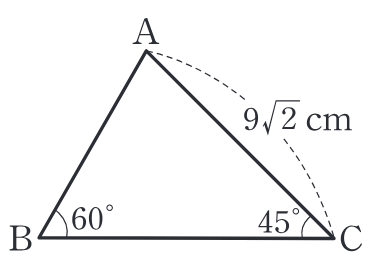
\includegraphics[width=\dmfigw]{figures/fig-0192.png}\end{minipage}\par
